%%% LaTeX Template: Two column article
%%%
%%% Source: http://www.howtotex.com/
%%% Feel free to distribute this template, but please keep to referal to http://www.howtotex.com/ here.
%%% Date: February 2011

%%% Preamble
\documentclass[	DIV=calc,%
							paper=a4,%
							fontsize=10pt]{scrartcl}	 					% KOMA-article class

%\usepackage{lipsum}													% Package to create dummy text

\usepackage[italian]{babel}										% English language/hyphenation
\usepackage[protrusion=true,expansion=true]{microtype}				% Better typography
\usepackage{amsmath,amsfonts,amsthm}					% Math packages
\usepackage[pdftex]{graphicx}									% Enable pdflatex
\usepackage[svgnames]{xcolor}									% Enabling colors by their 'svgnames'
\usepackage[hang, small,labelfont=bf,up,textfont=it,up]{caption}	% Custom captions under/above floats
\usepackage{epstopdf}												% Converts .eps to .pdf
\usepackage{subfig}													% Subfigures
\usepackage{booktabs}												% Nicer tables
\usepackage{fix-cm}													% Custom fontsizes
% let break long bold, italic and uderlied lines
\usepackage{soul}
\usepackage[margin=1in]{geometry}

\usepackage[sfdefault]{quattrocento}
\usepackage[T1]{fontenc}

\usepackage[utf8]{inputenc}
\usepackage{upquote}

% Overwrite \begin{figure}[htbp] with \begin{figure}[H]
\usepackage{float}
\let\origfigure=\figure
\let\endorigfigure=\endfigure
\renewenvironment{figure}[1][]{%
   \origfigure[H]
}{%
   \endorigfigure
}

\definecolor{myblue}{HTML}{69a8d9}
\definecolor{mygray}{HTML}{666666}
\definecolor{mygraylight}{HTML}{eeeeee}

\fontencoding {OT1}
\fontfamily {phv}
%\usefont{OT1}{phv}{b}{n}
%\fontseries {m}
\fontshape {n}
%\fontsize {11pt} {19pt}
%\linespread {1}
\selectfont

% use upquote if available, for straight quotes in verbatim environments
\IfFileExists{upquote.sty}{\usepackage{upquote}}{}


\usepackage{graphicx}
% Redefine \includegraphics so that, unless explicit options are
% given, the image width will not exceed the width or the height of the page.
% Images get their normal width if they fit onto the page, but
% are scaled down if they would overflow the margins.
\makeatletter
\def\ScaleWidthIfNeeded{%
 \ifdim\Gin@nat@width>\linewidth
    \linewidth
  \else
    \Gin@nat@width
  \fi
}
\def\ScaleHeightIfNeeded{%
  \ifdim\Gin@nat@height>0.9\textheight
    0.9\textheight
  \else
    \Gin@nat@width
  \fi
}
\makeatother

\setkeys{Gin}{width=\ScaleWidthIfNeeded,height=\ScaleHeightIfNeeded,keepaspectratio}%



% use microtype if available
\IfFileExists{microtype.sty}{%
\usepackage{microtype}
\UseMicrotypeSet[protrusion]{basicmath} % disable protrusion for tt fonts
}{}

\usepackage{ifxetex,ifluatex}
\ifxetex
  \usepackage[setpagesize=false, % page size defined by xetex
              unicode=false, % unicode breaks when used with xetex
              xetex]{hyperref}
\else
  \usepackage[unicode=true]{hyperref}
\fi
\hypersetup{breaklinks=true,
            bookmarks=true,
            pdfauthor={},
            pdftitle={A Markdown workflow for writing documents},
            colorlinks=true,
            citecolor=myblue,
            urlcolor=myblue,
            linkcolor=myblue,
            pdfborder={0 0 0}}
\urlstyle{same}  % don't use monospace font for urls
% let long URL breaking
\usepackage[anythingbreaks]{breakurl}

%%% Custom sectioning (sectsty package)
\usepackage{sectsty}													% Custom sectioning (see below)
\allsectionsfont{%															% Change font of al section commands
	\usefont{OT1}{phv}{b}{n}%										% bch-b-n: CharterBT-Bold font
	\color{myblue}% color
    \fontsize{20}{25}
    }

\sectionfont{%																% Change font of \section command
	\usefont{OT1}{phv}{b}{n}%										% bch-b-n: CharterBT-Bold font
	\color{myblue}% color
    \fontsize{20}{25}
	}

\chapterfont{
	\usefont{OT1}{phv}{b}{n}%										% bch-b-n: CharterBT-Bold font
    \color{myblue}
    }  % sets colour of chapters

%%% Headers and footers
\usepackage{fancyhdr}												% Needed to define custom headers/footers
	\pagestyle{fancy}														% Enabling the custom headers/footers
\usepackage{lastpage}	

% Header (empty)
\lhead{\emph{A Markdown workflow for writing documents}}
\chead{}
%\rhead{}
\rhead{
\includegraphics[width=1.5cm]{img/logo.png}}
% Footer (you may change this to your own needs)
\lfoot{\footnotesize {http://www.bertera.it} \copyright\ 2015 Bertera Pietro}
\cfoot{}
\rfoot{\footnotesize pagina \thepage\ di \pageref*{LastPage}}	% "Page 1 of 2"
\renewcommand{\headrulewidth}{1pt}
\renewcommand{\footrulewidth}{1pt}
\newcommand{\headrulecolor}[1]{\patchcmd{\headrule}{\hrule}{\color{#1}\hrule}{}{}}
\newcommand{\footrulecolor}[1]{\patchcmd{\footrule}{\hrule}{\color{#1}\hrule}{}{}}
\footrulecolor{mygray}
\headrulecolor{mygray}

% abstract environment

\usepackage{tcolorbox}
%\colorlet{shadecolor}{mygraylight}
%\colorlet{framecolor}{myblue}
%\renewenvironment{abstract}{ %
%    \def\FrameCommand{\fboxrule=\FrameRule\fboxsep=\FrameSep \fcolorbox{framecolor}{shadecolor}}%
%    \MakeFramed {\FrameRestore}}%
%    {\endMakeFramed}
\renewenvironment{abstract}
  {\begin{tcolorbox}[colframe=myblue,colback=mygraylight]}
  {\end{tcolorbox}}


%%% Creating an initial of the very first character of the content
\usepackage{lettrine}
\newcommand{\initial}[1]{%
     \lettrine[lines=3,lhang=0.3,nindent=0em]{
     				\color{DarkGoldenrod}
     				{\textsf{#1}}}{}}

%%% Title, author and date metadata
\usepackage{titling}															% For custom titles

\newcommand{\HorRule}{\color{mygray}%			% Creating a horizontal rule
									  	\rule{\linewidth}{1pt}%
								}

\pretitle{\vspace{-30pt} \begin{flushleft} %\HorRule 
				\fontsize{30}{50} \usefont{OT1}{phv}{b}{n} \color{myblue} \selectfont 
				}


\title{A Markdown workflow for writing documents}
\posttitle{\par\end{flushleft}\vskip 0.5em}

    \preauthor{\begin{flushright}
	    \large \lineskip 0.5em \usefont{OT1}{phv}{b}{sl} \color{mygray}
    }
    \author{bertera.it}
        \postauthor{\footnotesize \usefont{OT1}{phv}{m}{sl} \color{mygray} 
		\ Pietro Bertera
    	\par\end{flushright}
        \HorRule
    }

\date{April 2015}


% no indent for new paragraph and use one line of spacing
\usepackage[parfill]{parskip}

%%% Begin document
\begin{document}

\maketitle
\begin{abstract}
A plaintex, versionable, flexible authoring workflow using Markdown
\end{abstract}


\thispagestyle{fancy} 			% Enabling the custom headers/footers for the first page 

\section{A Markdown workflow for writing
documents}\label{a-markdown-workflow-for-writing-documents}

\subsection{Why Markdown ?}\label{why-markdown}

\begin{itemize}
\item
  \href{http://en.wikipedia.org/wiki/Markdown}{Markdown} is a simple and
  powerful formatting syntax, markdown has a flat learning curve
\item
  Markdown
  \href{http://brettterpstra.com/2011/08/31/why-markdown-a-two-minute-explanation/}{saves}
  time (and money): writing in markdown is fast: you musn't fight with a
  complicated syntax (read: LaTeX) nor you will never feel lost in a
  deep and deep XML tree (read: Docbook) and you will never need an
  heavy and buggy WYSIWYG editor.
\item
  Markdown is
  \href{https://help.github.com/articles/markdown-basics/}{plaintext},
  so you can use your preferred text editor: showing differences between
  documents is easy and you can use some tool (diff). Your document can
  be easily managed by any SCM tool (GIT, SVN, CVS, \ldots{})
\item
  Markdown is
  \href{http://mashable.com/2013/06/24/markdown-tools/}{portable}: you
  can write your docs in your smartphone, in your web editor or in your
  standalone application. Your markdown files will never be obsolete or
  unsupported.
\item
  Markdown is \href{https://stackedit.io/}{human readable}: also without
  any rendering process a markdown file is clean and easy to understand.
\item
  Markdown is \href{http://pandoc.org/}{flexible}: you can easily
  convert a Markdown document into an HTML, a PDF a DOCX or whatever in
  a few simple step and using numerous tools.
\item
  Markdown supports
  \href{http://programminghistorian.org/lessons/sustainable-authorship-in-plain-text-using-pandoc-and-markdown}{workflows}:
  with some tools and a simple setup you can automatize your
  writing-release-publish-print-backup-upload-whatever process: you can
  script the rendering process, or the publishing and so on.
\end{itemize}

\section{The workflow}\label{the-workflow}

My workflow is based on a Makefile and consist in a few automated steps:

\begin{itemize}
\itemsep1pt\parskip0pt\parsep0pt
\item
  copy all the markdown files into the \emph{gen/\{format\}/} (format is
  your product format (html, pdf, docx, \ldots{} )
\item
  convert all images using the appropriate rule (see below) into the
  \emph{gen/\{format\}/img/} directory
\item
  copy all the needed templates into the \emph{gen/\{format\}/tpl}
  directory
\item
  run \emph{pandoc} inside the \emph{gen/\{format\}/} directory in order
  to create the output document
\end{itemize}

\section{Images resize issue}\label{images-resize-issue}

One of the Markdown drawbacks is that doesn't officially supports an
image resizing syntax.

This limitation is due by the fact that often the wanted image size
depends on the final document format. If your document is rendered as
HTML maybe you want bigger images than in A4 PDF rendering.

This limitation can be circumvented using little script and a rule file:
the rule file resides along with the file and has a the same name of the
image file followed by the suffix \texttt{.sizes} E.g.: the image
\textbf{tls-enforcing.png} has a rule file named
\textbf{tls-enforcing.png.sizes}.

The rule file contains a list of
\href{http://www.imagemagick.org/script/convert.php}{convert} options
grouped by format:

\subsection{Example:
\textbf{tls-enforcing.png.sizes}}\label{example-tls-enforcing.png.sizes}

\begin{verbatim}
# This is a comment and will be ignored during the parsing
# The following rule instructs the convert tool to resize 
# the image to the specified size
pdf:-resize 400x50
# The following rule specify a width of 300px for the HTML format
html:-resize 300
# All others format should be unchanged
ALL:
\end{verbatim}

\subsubsection{The \emph{convert-img.sh}
script:}\label{the-convert-img.sh-script}

This bash script should be launched with 4 command line arguments:

\begin{itemize}
\itemsep1pt\parskip0pt\parsep0pt
\item
  the image file path
\item
  the needed format
\item
  a directory where the image should copied (after processed by
  \emph{convert})
\end{itemize}

When the script runs it search for the rule file, the rule file is
parsed against the format and then the convert command is launched with
the format specific options.

So, running the script:

\texttt{./scripts/onvert-img.sh img/tls-enforcing.png pdf gen/pdf/img}

The following command will be launched:

\texttt{convert -resize 400x50 img/tls-enforcing.png gen/pdf/img/tls-enforcing.png}

In case the rule file is missing or the rule file doesn't contains the
needed format the script will search for a fallback rule file named
\textbf{fallback.sizes}. In case the fallback file is missing image will
be copied withouth modifications into the destination directory.

\section{The working tree}\label{the-working-tree}

Following my working directory:

\begin{verbatim}
.
|____img/                           <--- *img*: the image directory          
| |____tls-unknown.png                   containing all images
| |____tls-unknown.png.sizes             along with rule files
| |____8021p.png
| |____tls-enforcing.png
| |____tls-enforcing.png.sizes
| |____vlan-wireshark.png
| |____fallback.sizes               <--- fallback rules file
|
|____Makefile                       <--- the Makefile
|
|____Networking.md                  <--- Markdown documents
|____Security.md
|____README.md
|
|____scripts/                       <--- Scripts directory containing
| |____convert-img.sh                    the convert-img.sh script 
|
|____tpl/                           <--- a template directory containing
| |____Byword.css                        stylesheets, html templates
| |____kultiad-serif.css                 LaTeX templates etc...
| |____latex.template
| |____latex.tex
| |____paper.css
| |____style.css
| |____template.html
| |____template.tex
\end{verbatim}

\section{Editing}\label{editing}

You can use your \href{http://www.vim.org/}{preferred} text
\href{http://www.gnu.org/software/emacs/}{editor}, I like to use
\href{http://mouapp.com/}{Mou}:

\begin{figure}[htbp]
\centering
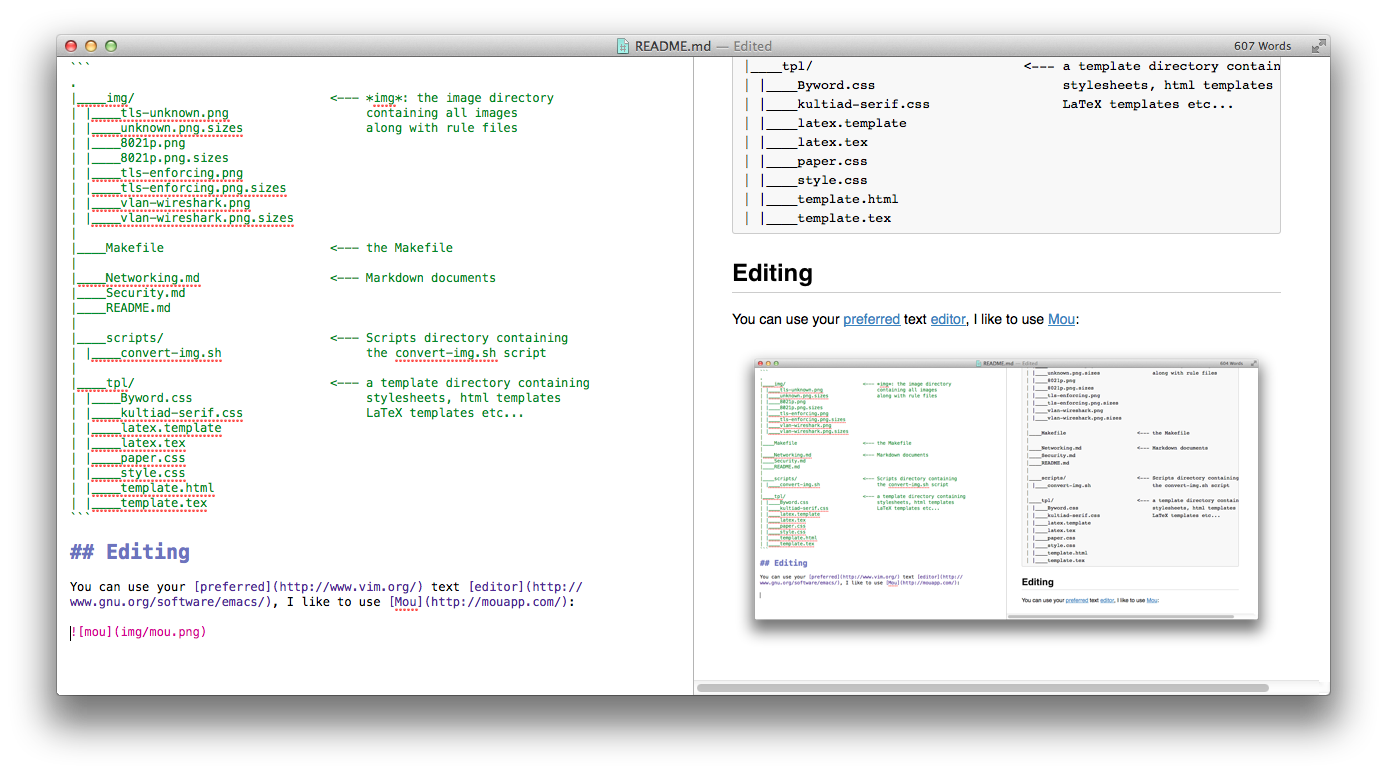
\includegraphics{img/mou.png}
\caption{The mou editor}
\end{figure}

\section{Generating the output
document}\label{generating-the-output-document}

The output document can be easily generated trough the \emph{GNU/Make}
command:

\texttt{make html}

Will generate an HTML document into the gen/html/ directory for each
Markdown document into the main directory:

\begin{verbatim}
gen/html/
|____img
|    |____tls-unknown.png
|    |____8021p.png
|    |____tls-enforcing.png
|    |____vlan-wireshark.png
|
|____tpl
|    |____style.css
|    |____template.html
|
|____Networking.html
|____README.html
|____security.html
\end{verbatim}

Same thing for \emph{make pdf} and \emph{make docx} commands. \emph{make
all} command will export HTML, PDF and DOCX formats.

You can easily configure the whole workflow editing the \emph{Makefile}
and format templates.

\section{Needed tools:}\label{needed-tools}

\subsection{ImageMagick}\label{imagemagick}

\href{http://www.imagemagick.org/}{ImageMagick} s a software suite to
create, edit, compose, or convert bitmap images. It can read and write
images in a variety of formats (over 200) including PNG, JPEG,
JPEG-2000, GIF, TIFF, DPX, EXR, WebP, Postscript, PDF, and SVG. Use
ImageMagick to resize, flip, mirror, rotate, distort, shear and
transform images, adjust image colors, apply various special effects, or
draw text, lines, polygons, ellipses and Bézier curves.

ImageMagick is used by the \emph{convert-img.sh} script.

\subsection{LaTex}\label{latex}

You need a full working LaTex environment installed. Nedded packages
depends from your LaTex template.

\subsection{Pandoc}\label{pandoc}

\href{http://johnmacfarlane.net/pandoc/}{Pandoc} is a universal document
converter. It works from the command line and you can quickly convert a
document between any two formats. These include nearly all formats
commonly used for scientific writing such as Word, Markdown, ODT, LaTeX,
HTML and RTF.

\href{http://johnmacfarlane.net/pandoc/installing.html}{Download and
install pandoc}

\subsection{Cool Markdown editors:}\label{cool-markdown-editors}

\subsubsection{Texts}\label{texts}

\href{http://www.texts.io}{Texts} is rich editor for Markdown, with
multiple export options (e.g.~PDF, Microsoft Word, LaTeX, HTML, ePub)
for OS X and Windows.

\subsubsection{ByWord}\label{byword}

\href{http://www.bywordapp.com}{ByWord} is a simple text editor for OS X
and iOS.

\subsubsection{Mou}\label{mou}

\href{http://mouapp.com}{Mou} is a simple, free, and powerful Markdown
editor/previewer for OS X.

\subsubsection{MarkdownPad}\label{markdownpad}

\href{http://markdownpad.com/}{MarkdownPad} is a Markdown editor for
Windows. Both a Free and a Pro version exist; the latter adds support
for (amongst other things) GitHub Flavored Markdown and Markdown Extra
(including Tables).

\subsubsection{MultiMarkdown Composer}\label{multimarkdown-composer}

``\href{http://multimarkdown.com}{MultiMarkdown Composer} is a text
editor for Mac that is designed from the ground up around the
MultiMarkdown Syntax. It is designed to make writing in MultiMarkdown
(or Markdown) even easier than it already is, with automatic syntax
highlighting, built in previews, easy export to any format that is
supported by MultiMarkdown, and more!'' {[}http://multimarkdown.com{]}.

\subsubsection{ReText}\label{retext}

\href{http://sourceforge.net/p/retext/home/ReText/}{ReText} is an
open-source, platform-independent editor for both Markdown and
reStructuredText.

\subsubsection{Qute}\label{qute}

\href{https://github.com/fbreuer/qute}{Qute}, is an open source,
platform-independent editor for Markdown with MathJax-integrated
live-preview.

\subsubsection{Erato}\label{erato}

\href{http://9muses.se/erato/}{Erato} is a markdown editor for Mac
users, supporting GitHub Flavored Markdown, including YAML front matter
and task lists.

\subsubsection{Editorial}\label{editorial}

\href{omz-software.com/editorial/}{Editorial} is a markdown editor app
for iOS users that includes inline markdown preview and is extensible
with workflows.

\subsubsection{Sublime Text}\label{sublime-text}

\href{http://www.sublimetext.com}{Sublime Text} is a text editor
available for OS X, Windows, and Linux. There are packages for working
with Markdown and Pandoc, notably
\href{https://packagecontrol.io/packages/MarkdownEditing}{MarkdownEditing}
and \href{https://packagecontrol.io/packages/Pandown}{Pandown}.

\subsubsection{Atom}\label{atom}

\href{https://atom.io/}{Atom} is a hackable text editor available for
Linux, OS X and Windows. It is completely open source, collaboratively
developed and maintained is GitHub. It supports
\href{https://help.github.com/articles/github-flavored-markdown/}{GitHub
Flavored Markdown} out of the box.

\subsubsection{Brackets}\label{brackets}

\href{http://brackets.io/}{Brackets} is an open source modern text
editor available for Linux, OS X and Windows by Adobe. It is
collaboratively developed and maintained on GitHub and has over 20,000
stargazers. Brackets supports markdown through

\href{http://blog.brackets.io/2013/04/23/markdown-extension-for-brackets/?lang=en}{Markdown}
\href{https://github.com/gruehle/MarkdownPreview}{Preview}
\href{https://brackets-registry.aboutweb.com/}{extension}. There is also
a \href{http://baig.github.io/brackets-zotero/}{Zotero Integration}
extension which lets you search and add citation keys in your scholarly
markdown documents from your local
\href{https://www.zotero.org/}{Zotero} library.

\subsection{Web-based editors}\label{web-based-editors}

\subsubsection{Zupadoc}\label{zupadoc}

\href{http://zupadoc.com}{Zupadoc} is a web-based markdown editor which
exports markdown text to typeset PDFs (articles and slides are
available). Integrates with Dropbox.

\subsubsection{Draft}\label{draft}

\href{https://draftin.com}{Draft} is a web-based markdown editor with
cloud sync, image hosting and analytics.

\subsubsection{Markable}\label{markable}

\href{http://markable.in/}{Markable} is another web-based markdown
editor with export and integration options.

\subsubsection{StackEdit}\label{stackedit}

\href{https://stackedit.io/editor}{StackEdit} is another markdown editor
with export and publishing options.

\subsubsection{Prose.io}\label{prose.io}

\href{http://prose.io}{Prose} is a web-based markdown editor for Github
Pages.

\subsubsection{Authorea}\label{authorea}

\href{https://www.authorea.com/}{Authorea} is an online collaborative
editor to write scientific, academic, and technical documents online and
includes markdown and Latex editing.

\subsection{Previewers}\label{previewers}

\subsubsection{Marked}\label{marked}

\href{http://markedapp.com}{Marked} is a markdown previewer for OS X.

\end{document}
